\newcommand{\outlierFig}{
  \begin{figure}
  \centering
  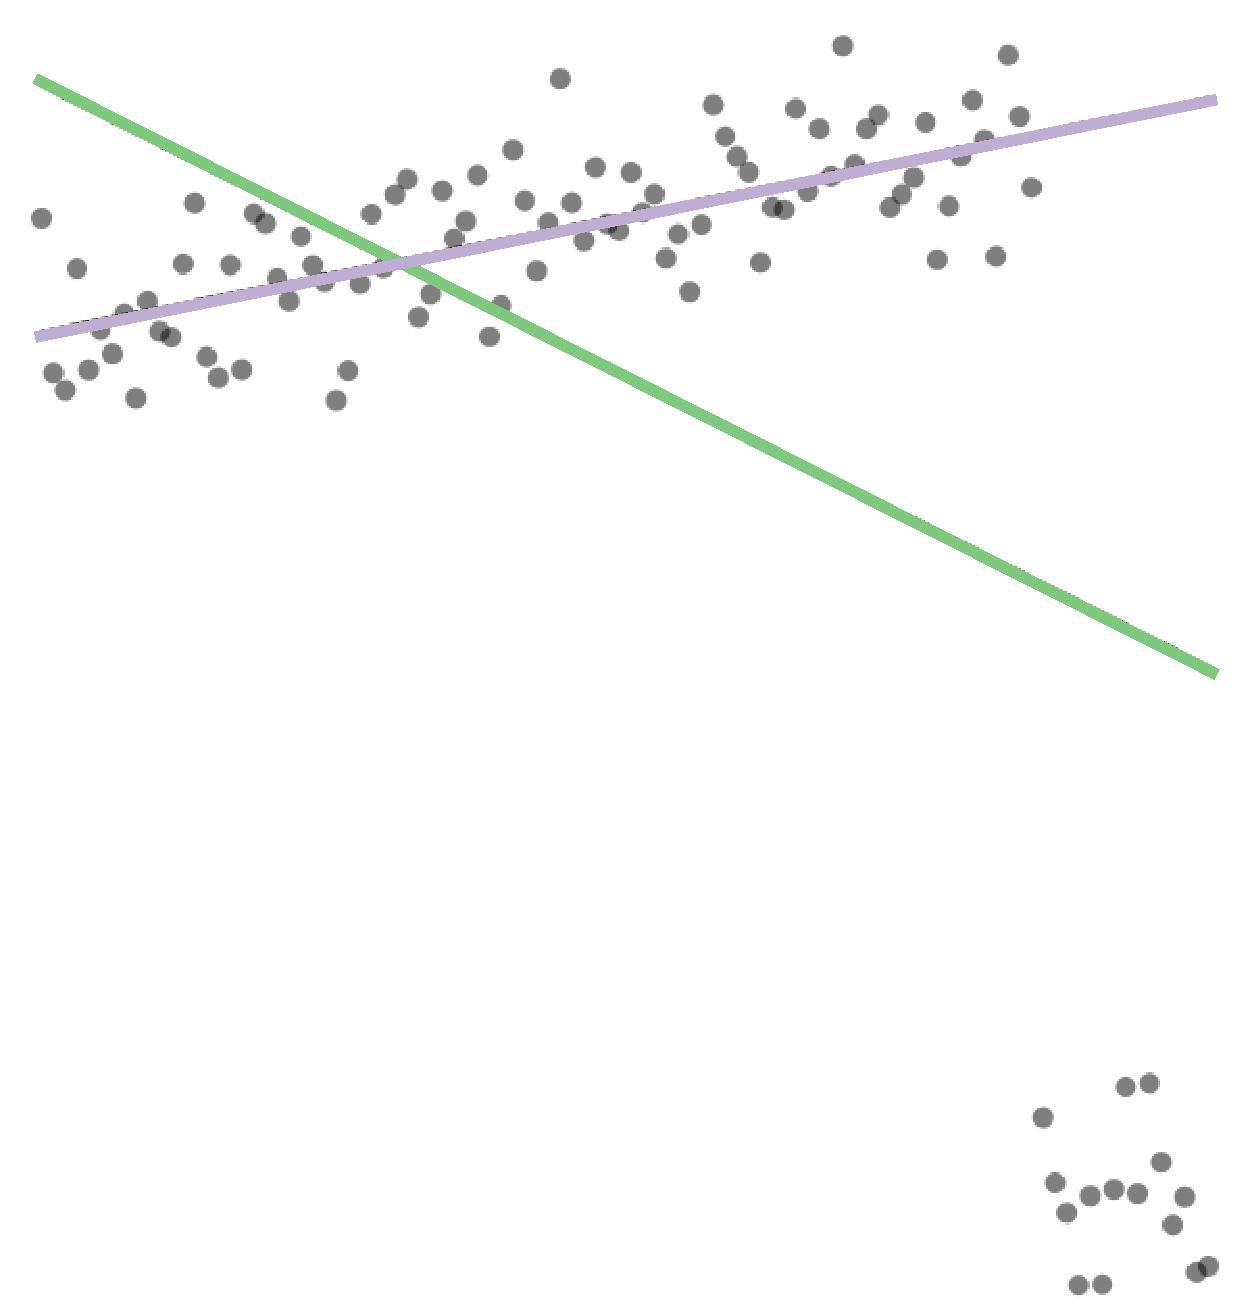
\includegraphics[width=.55\columnwidth]{figures/exp4}
  \caption{An example stimulus from Experiment 3. We replaced the final 10 points of this dataset with extreme values. The overlaid green trend line represents a robust fit (ignoring the outlier values), while the overlaid orange line represents the standard OLS fit with all points included. The purple line represents the average participant response on this stimulus. In general, participants' estimates of trend lines were closer to the robust than the non-robust trend; regression by eye tends to down-weight outliers compared to OLS.}
  \label{fig:outlier}
  \end{figure}
}

\newcommand{\outliersFig}{
	\begin{figure}
		\centering
		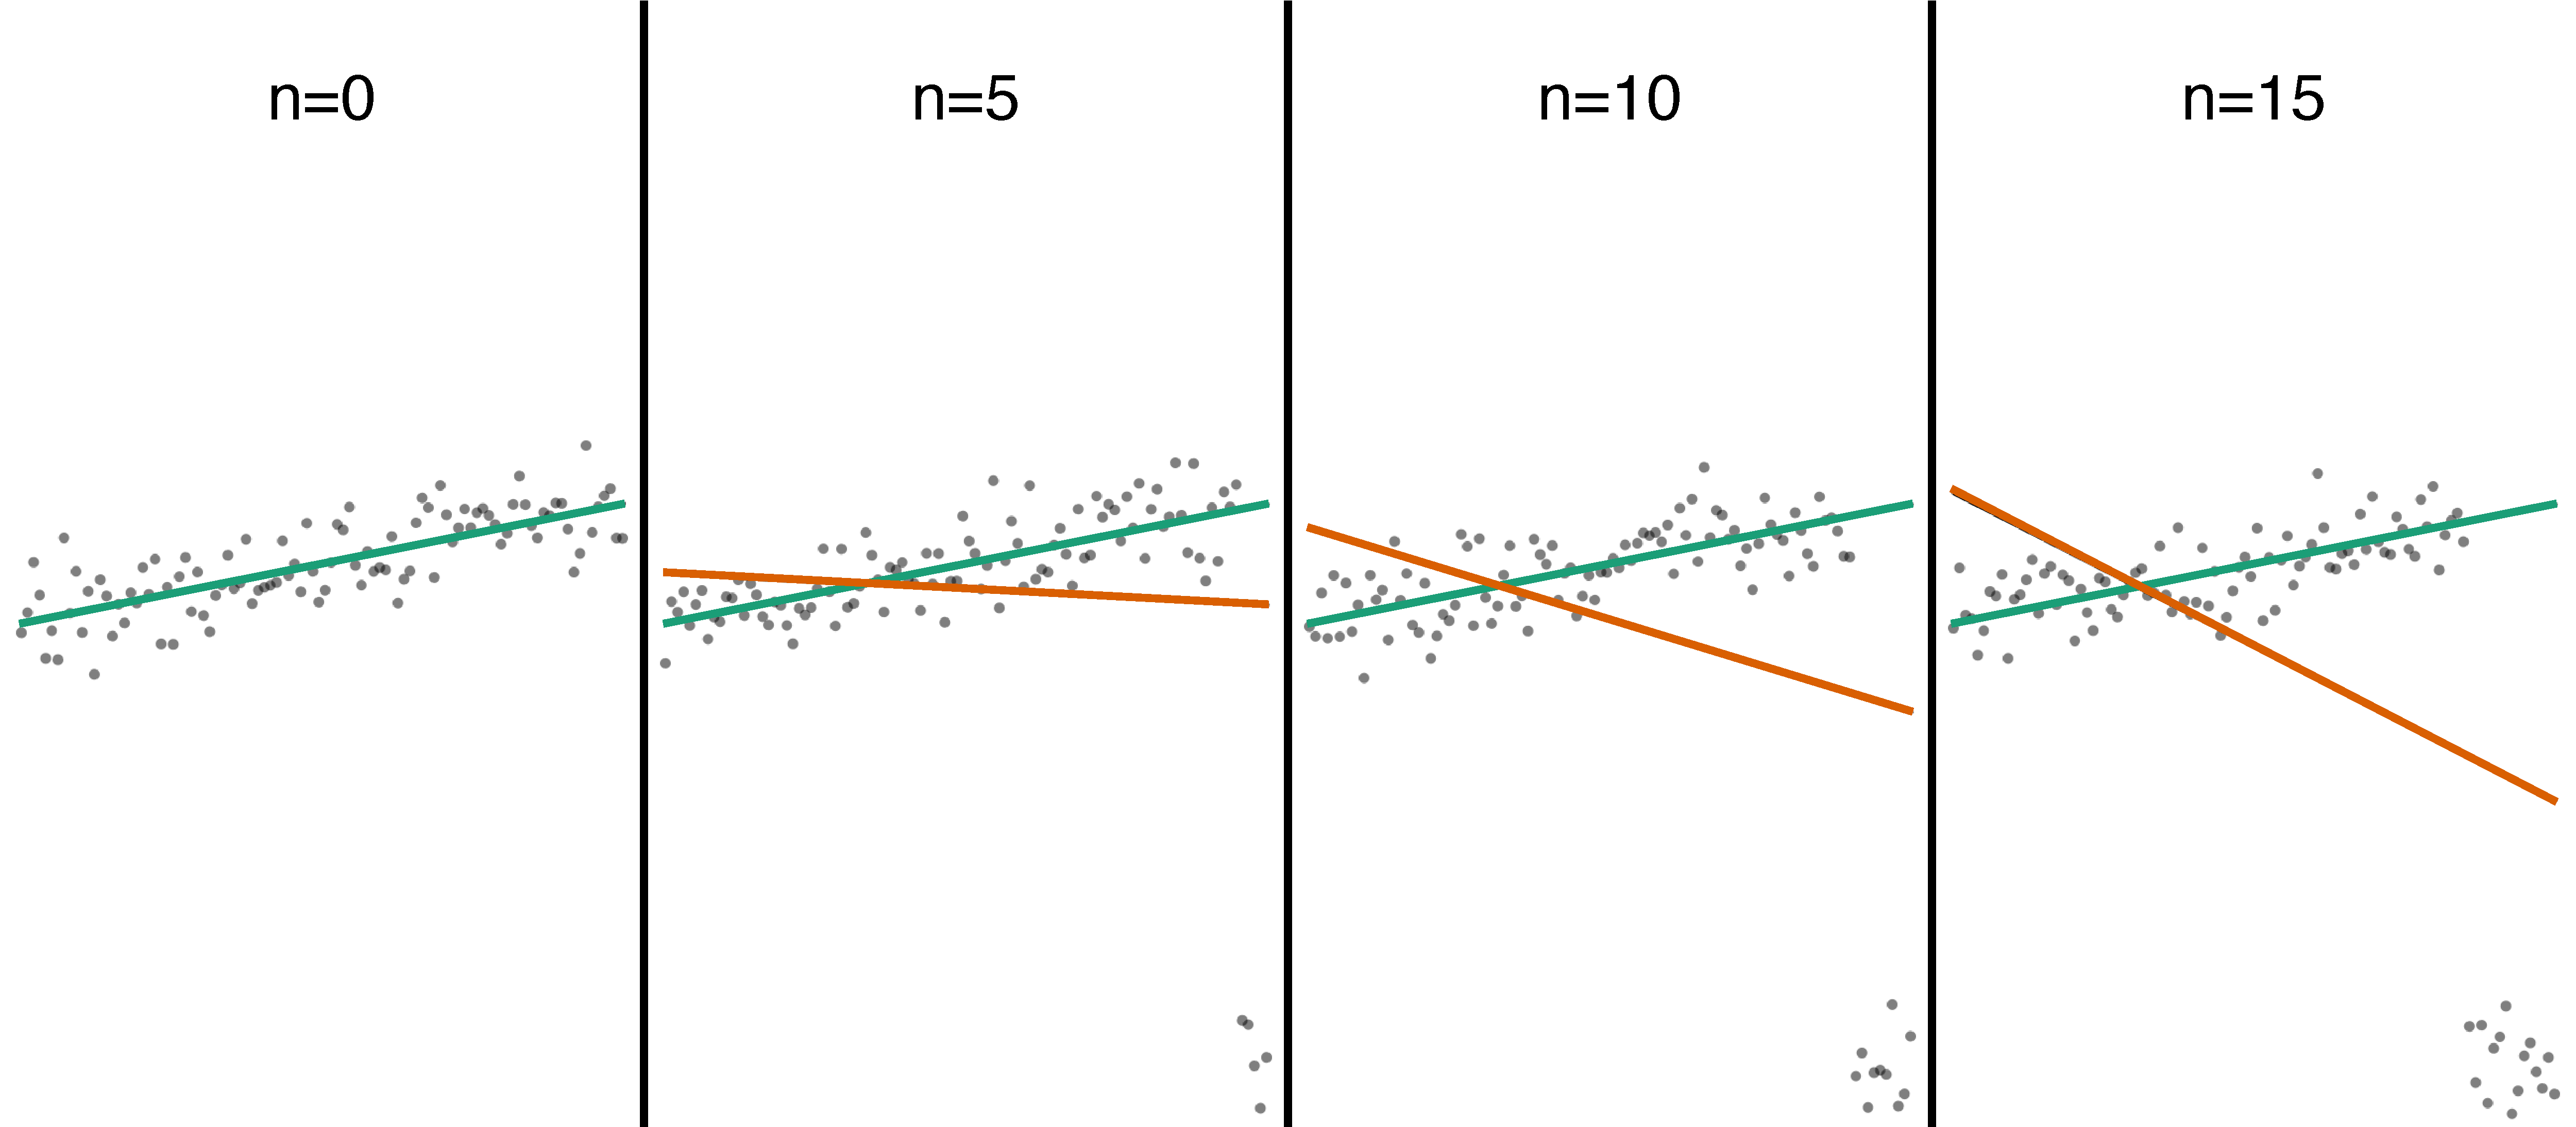
\includegraphics[width=.95\columnwidth]{figures/outliers}
		\caption{The four different outlier numerosities tested in Experiment 3. The overlaid green trend line represents a robust fit (ignoring the outlier values), while the overlaid orange line represents the standard OLS fit with all points included. More outliers results in larger divergence between these two types of fit.}
		\label{fig:outliers}
	\end{figure}
}

\newcommand{\expFig}{
  \begin{figure}
  \centering
  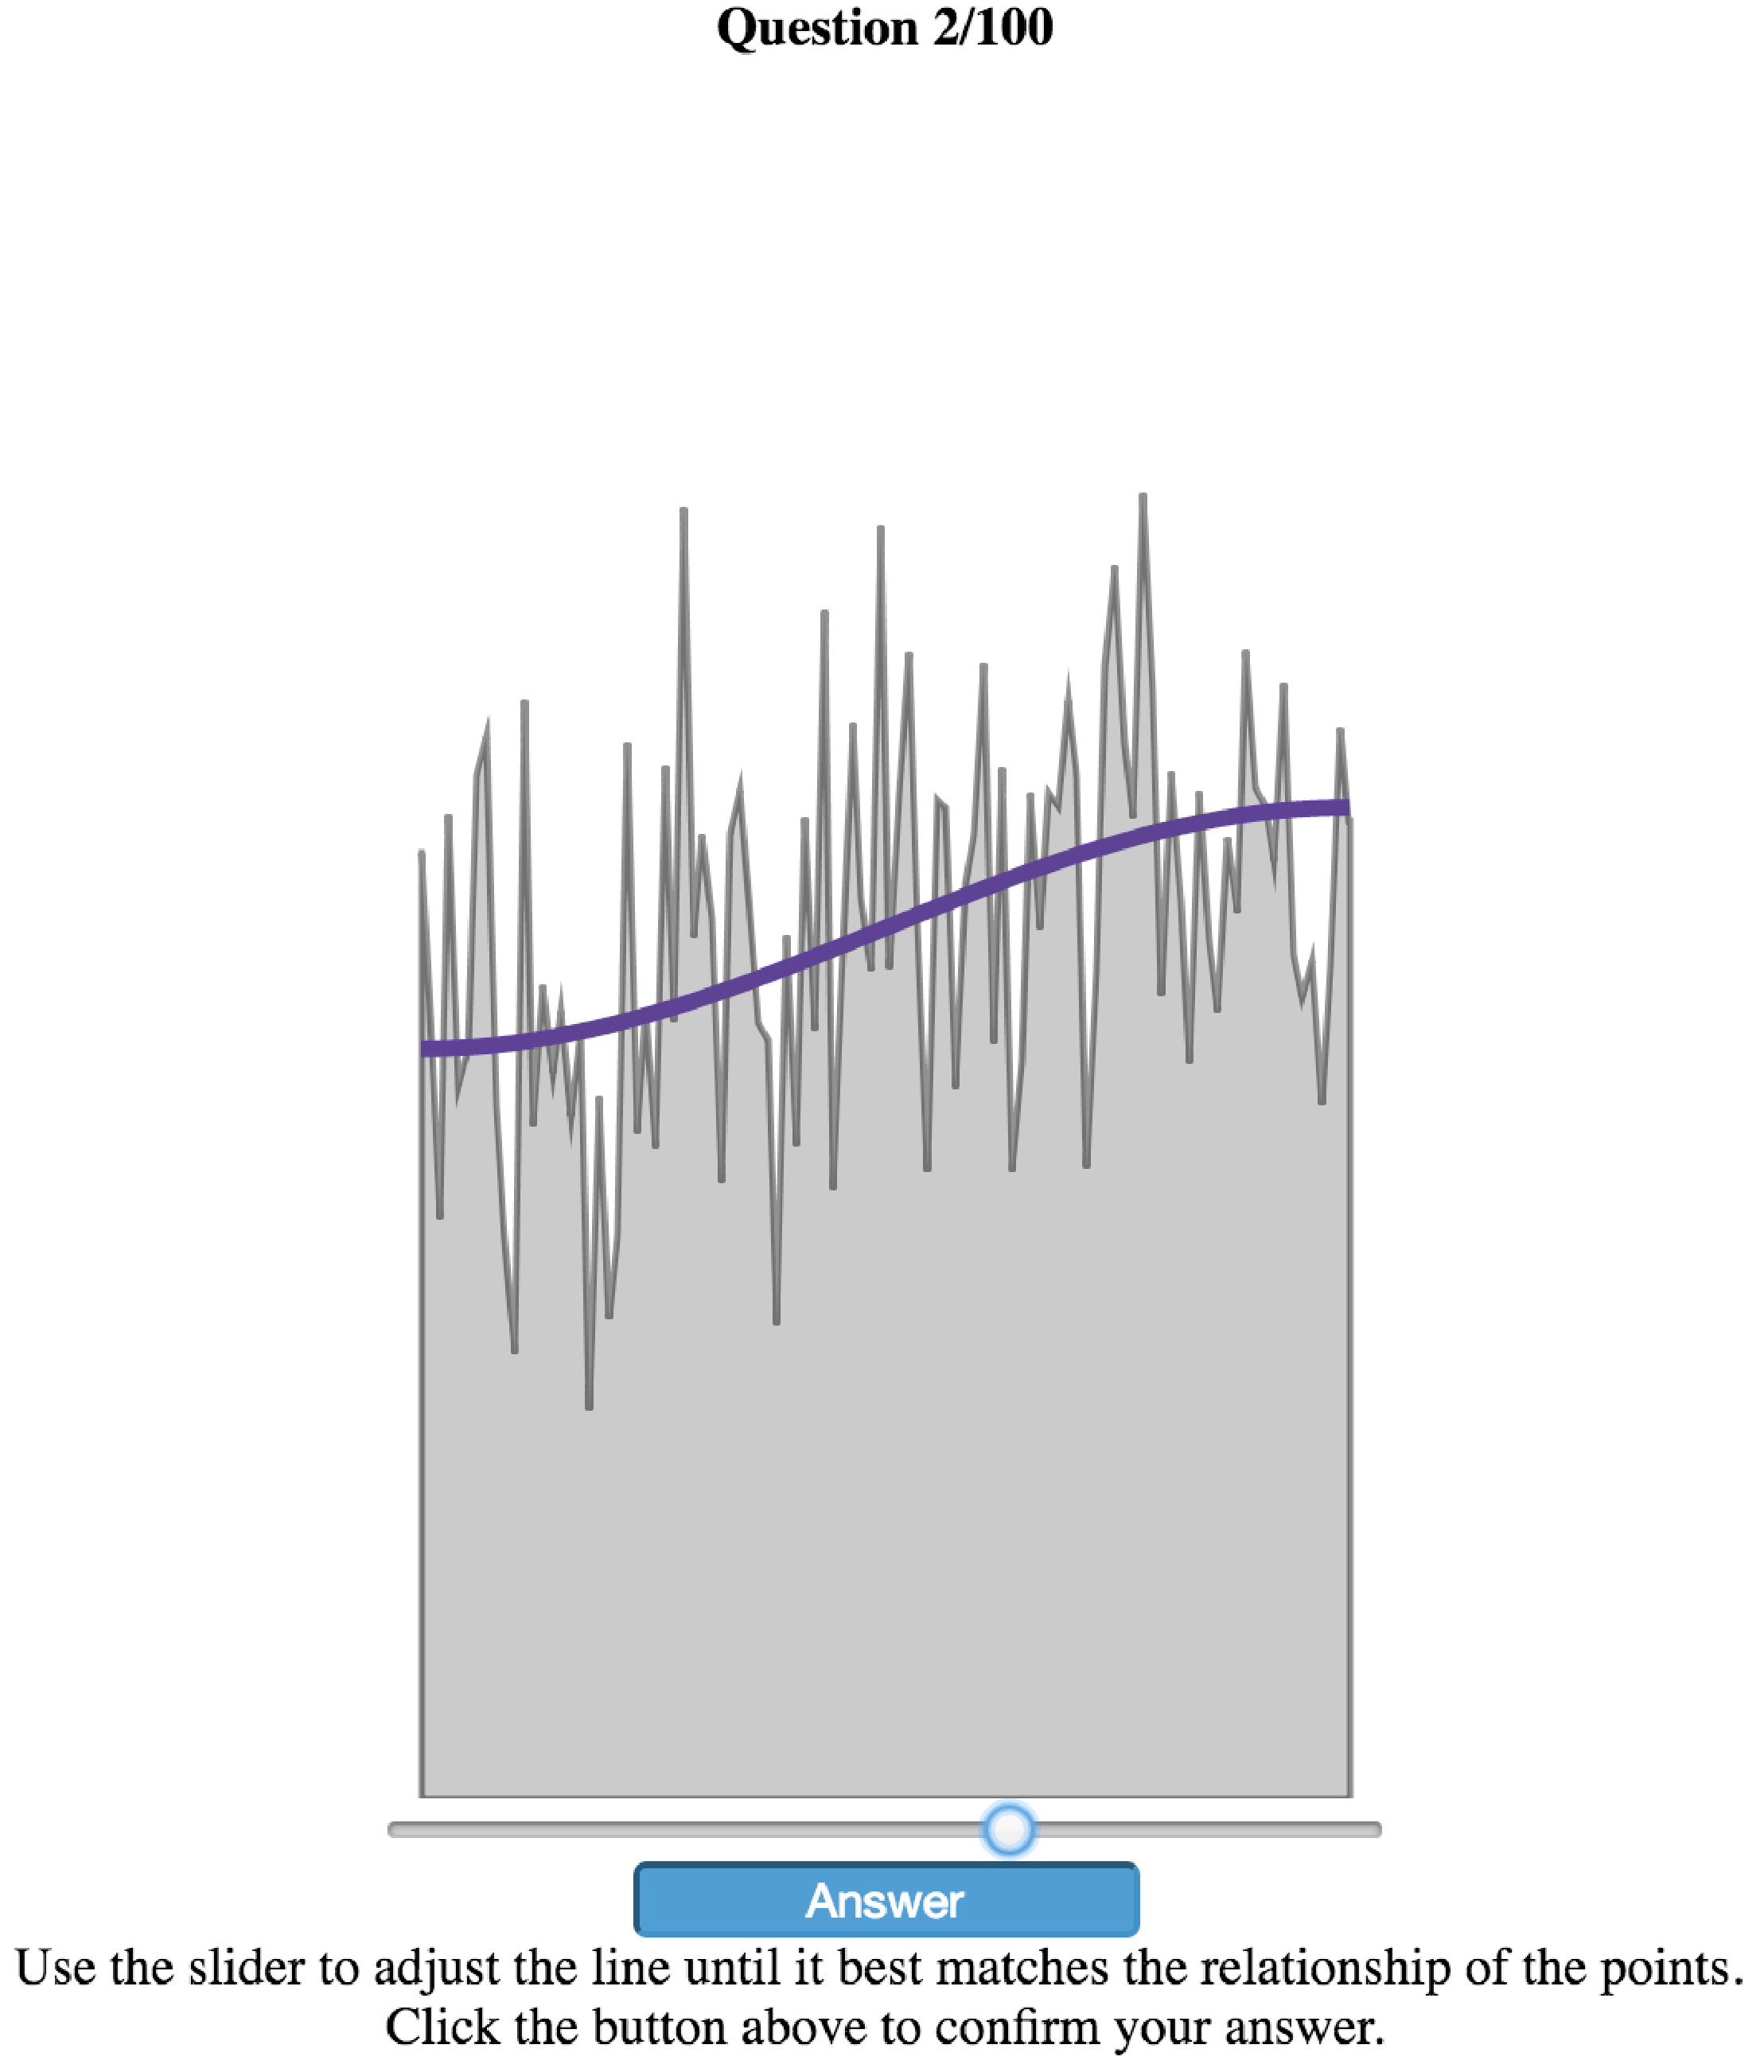
\includegraphics[width=1.0\columnwidth,trim={0 0 0 10cm},clip]{figures/exp}
  \caption{An example estimation task from our experiments. Here, the participant must adjust the amplitude of the purple trigonometric function until it best matches a particular set of bivariate data.}
  \label{fig:experiment}
  \end{figure}
}

\newcommand{\anscombeFig}{
	\begin{figure*}
		\centering
		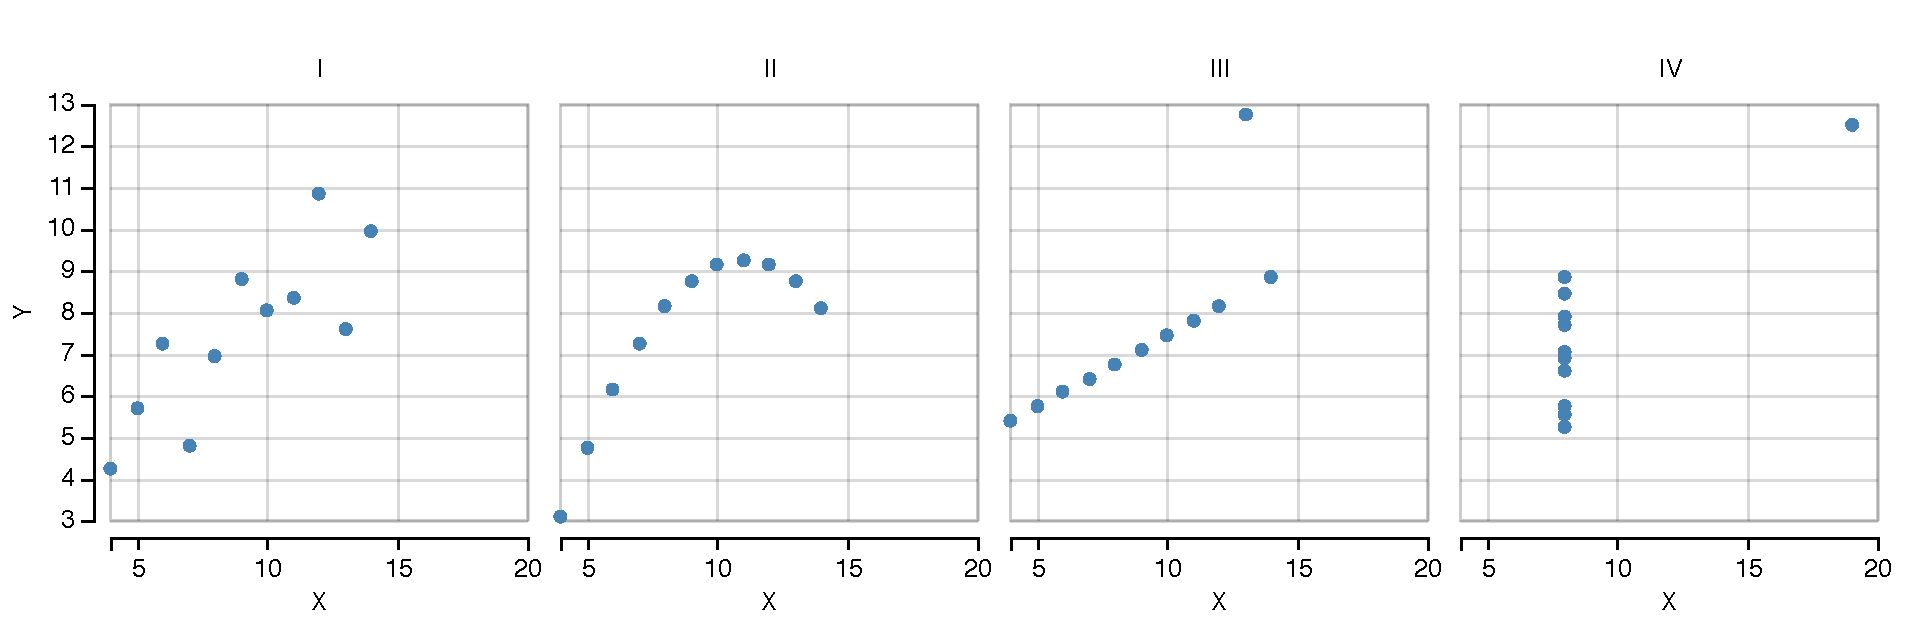
\includegraphics[width=.75\textwidth]{figures/anscombe}
		\caption{Anscombe's quartet. Each series has nearly identical summary statistics include mean, standard deviation, and linear fit. Yet, through visual inspection, viewers can disambiguate  differing patterns and trends. We refer to this visual estimation of trends as ``regression by eye.''}
		\label{fig:anscombe}
	\end{figure*}
}

\newcommand{\sigmasFig}{
	\begin{figure}
		\centering
		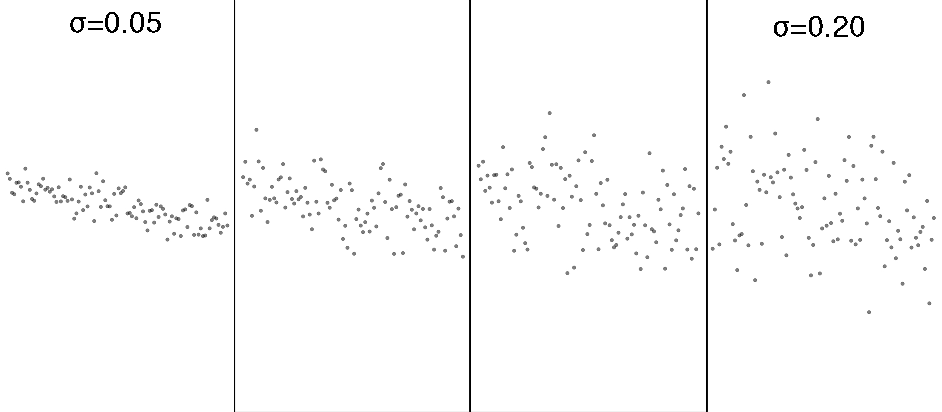
\includegraphics[width=.95\columnwidth]{figures/sigmas}
		\caption{The four different Gaussian bandwidths used to generate residuals in this study. We produced stimuli by creating points on a target trend line (in this case, $f(x) = -0.2x + 0.6$), and then adding residuals drawn evenly from a Gaussian with a given bandwidth $\sigma$. Larger bandwidths mean more dispersion and so weaker fits.}
		\label{fig:sigmas}
	\end{figure}
}

\newcommand{\trendtypesFig}{
	\begin{figure}
		\centering
		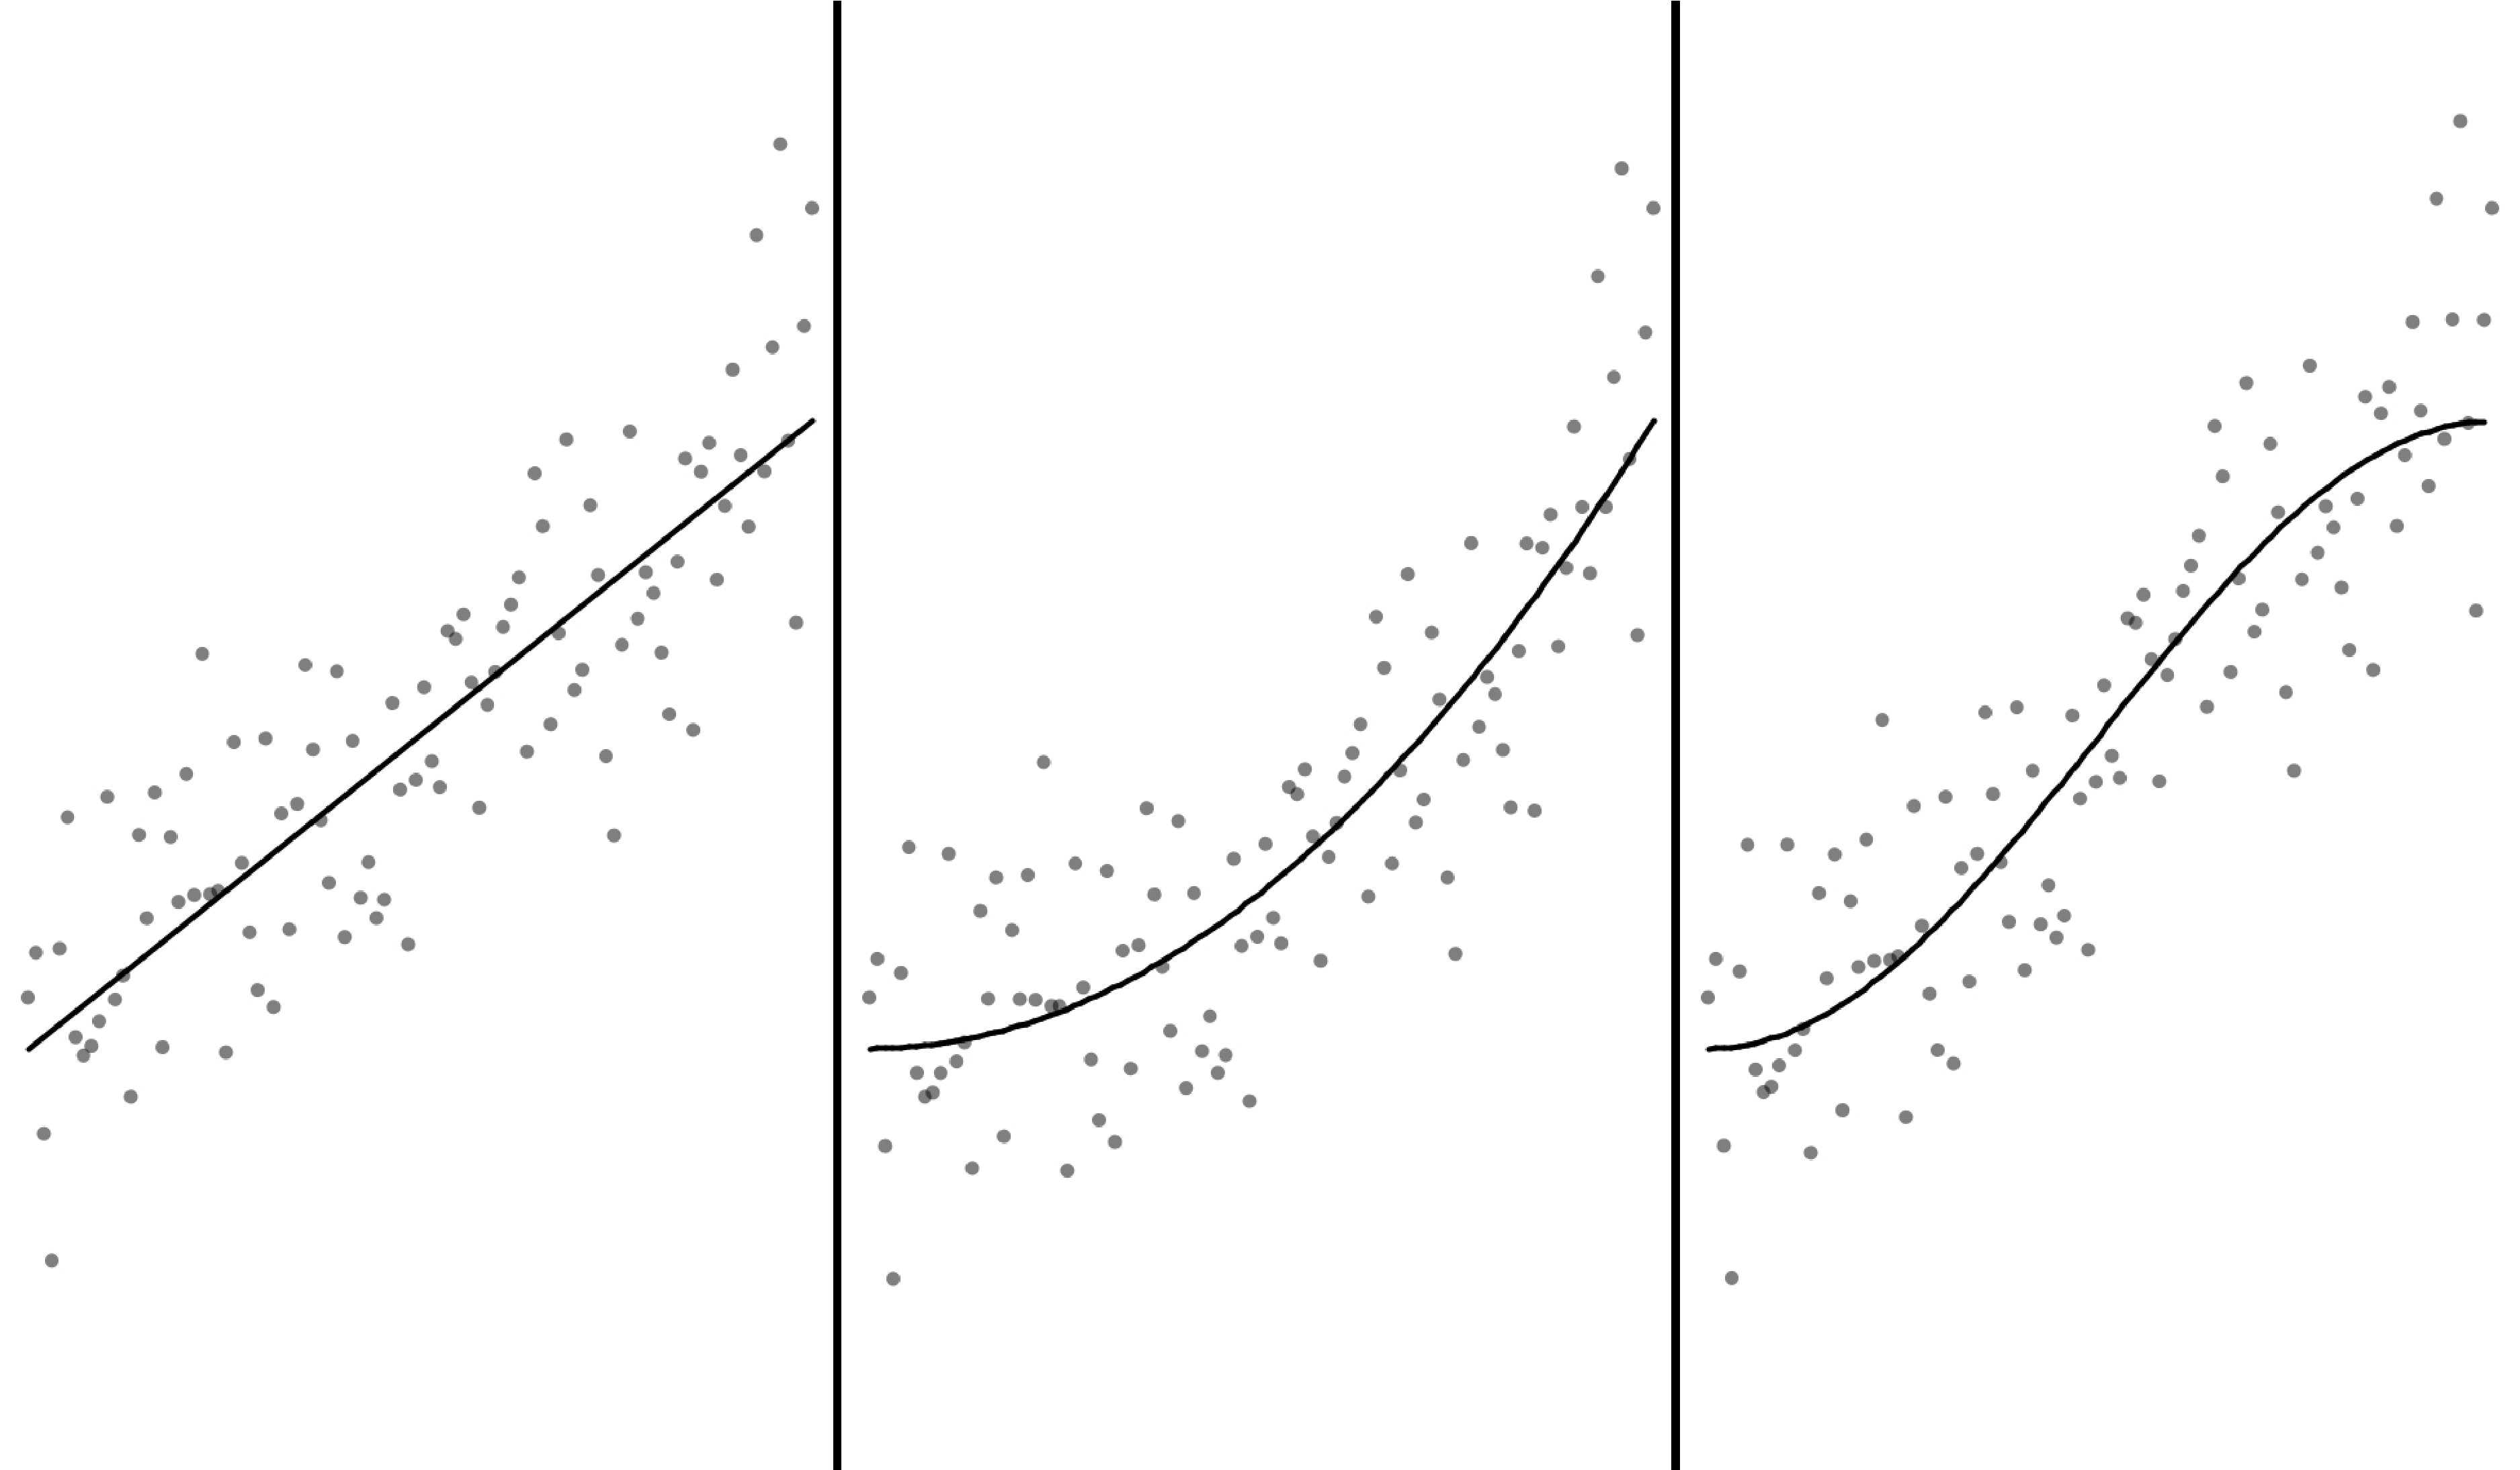
\includegraphics[width=.95\columnwidth]{figures/trendtypes}
		\caption{The three different trend types in this study: linear, quadratic, and trigonometric trends. In Experiment 1, participants estimated the slope of the linear fits, curvature of the quadratic fits, and amplitude of the trigonometric fits. In Experiment 2, they estimated the y-intercept of these fits. In Experiment 3, they estimated only the slope of linear fits. Trend lines are displayed here for reference. }
		\label{fig:trendtypes}
	\end{figure}
}

\newcommand{\expOnesigmasFig}{
	\begin{figure}
		\centering
		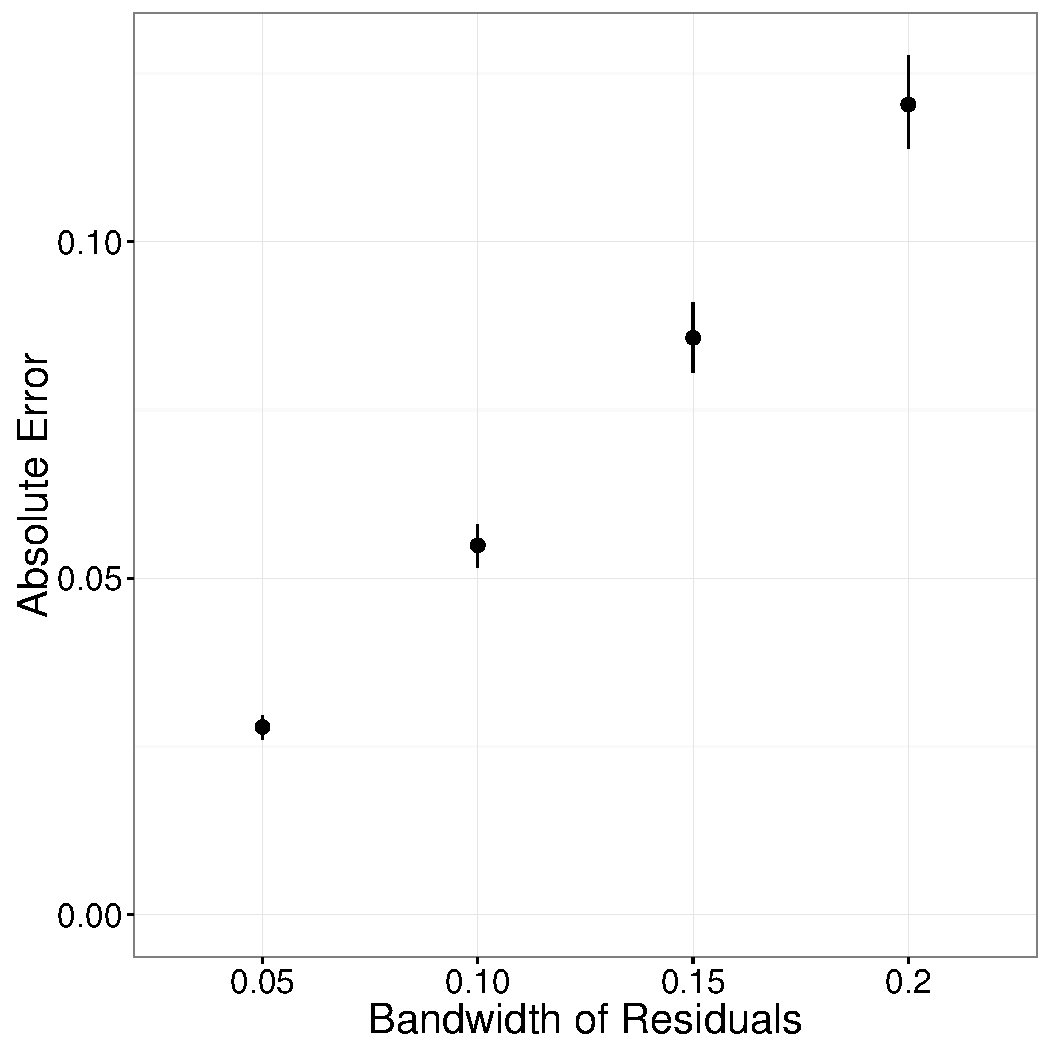
\includegraphics[width=.85\columnwidth]{figures/exp1sigmas}
		\caption{The effect of increased residual bandwidth on error in Experiment 1. See Fig. \protect\ref{fig:sigmas} for example stimuli at each factor level. Absolute error at estimating trend monotonically increases as the goodness of fit decreases. Confidence intervals represent bootstrapped 95\% CIs of interquartile means. }
		\label{fig:exp1sigmas}
	\end{figure}
}

\newcommand{\expOnetypesFig}{
	\begin{figure}
		\centering
		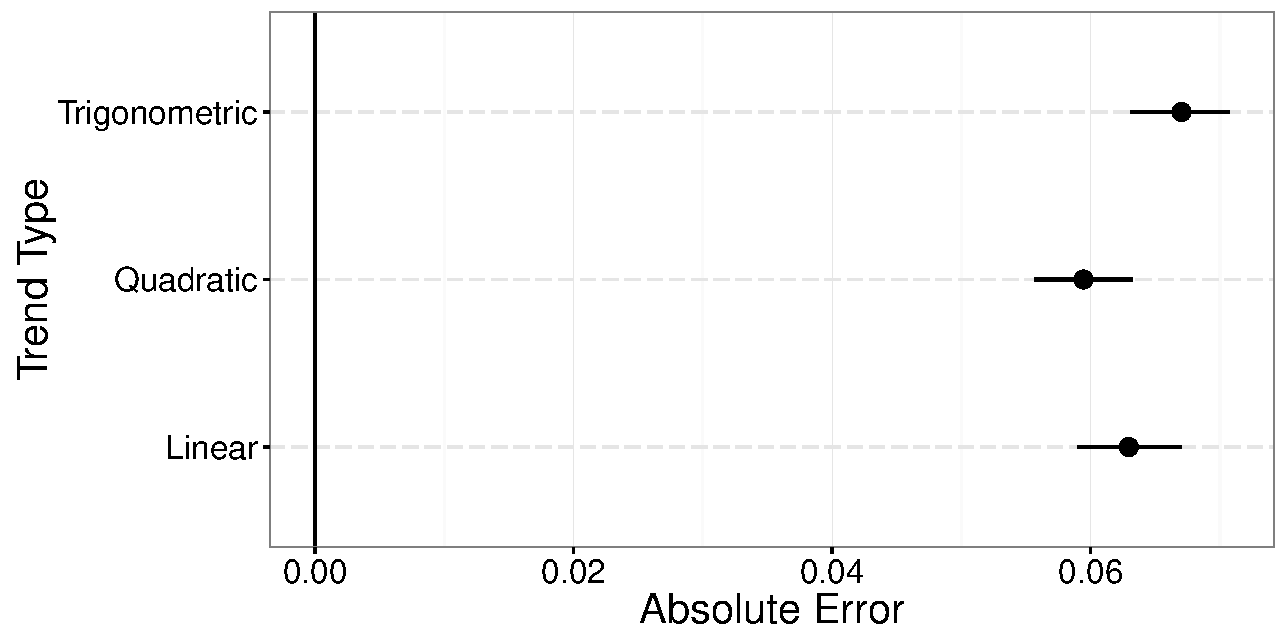
\includegraphics[width=.85\columnwidth]{figures/exp1types}
		\caption{The effect of different trend types on error in Experiment 1. See Fig. \protect\ref{fig:trendtypes} for example stimuli at each factor level. Despite the differing complexity of these types of fit, participant estimates were similar, indicating that regression by eye is capable of non-linear estimates. Confidence intervals represent bootstrapped 95\% CIs of interquartile means. }
		\label{fig:exp1types}
	\end{figure}
}

\newcommand{\typesFig}{
	\begin{figure}
		\centering
		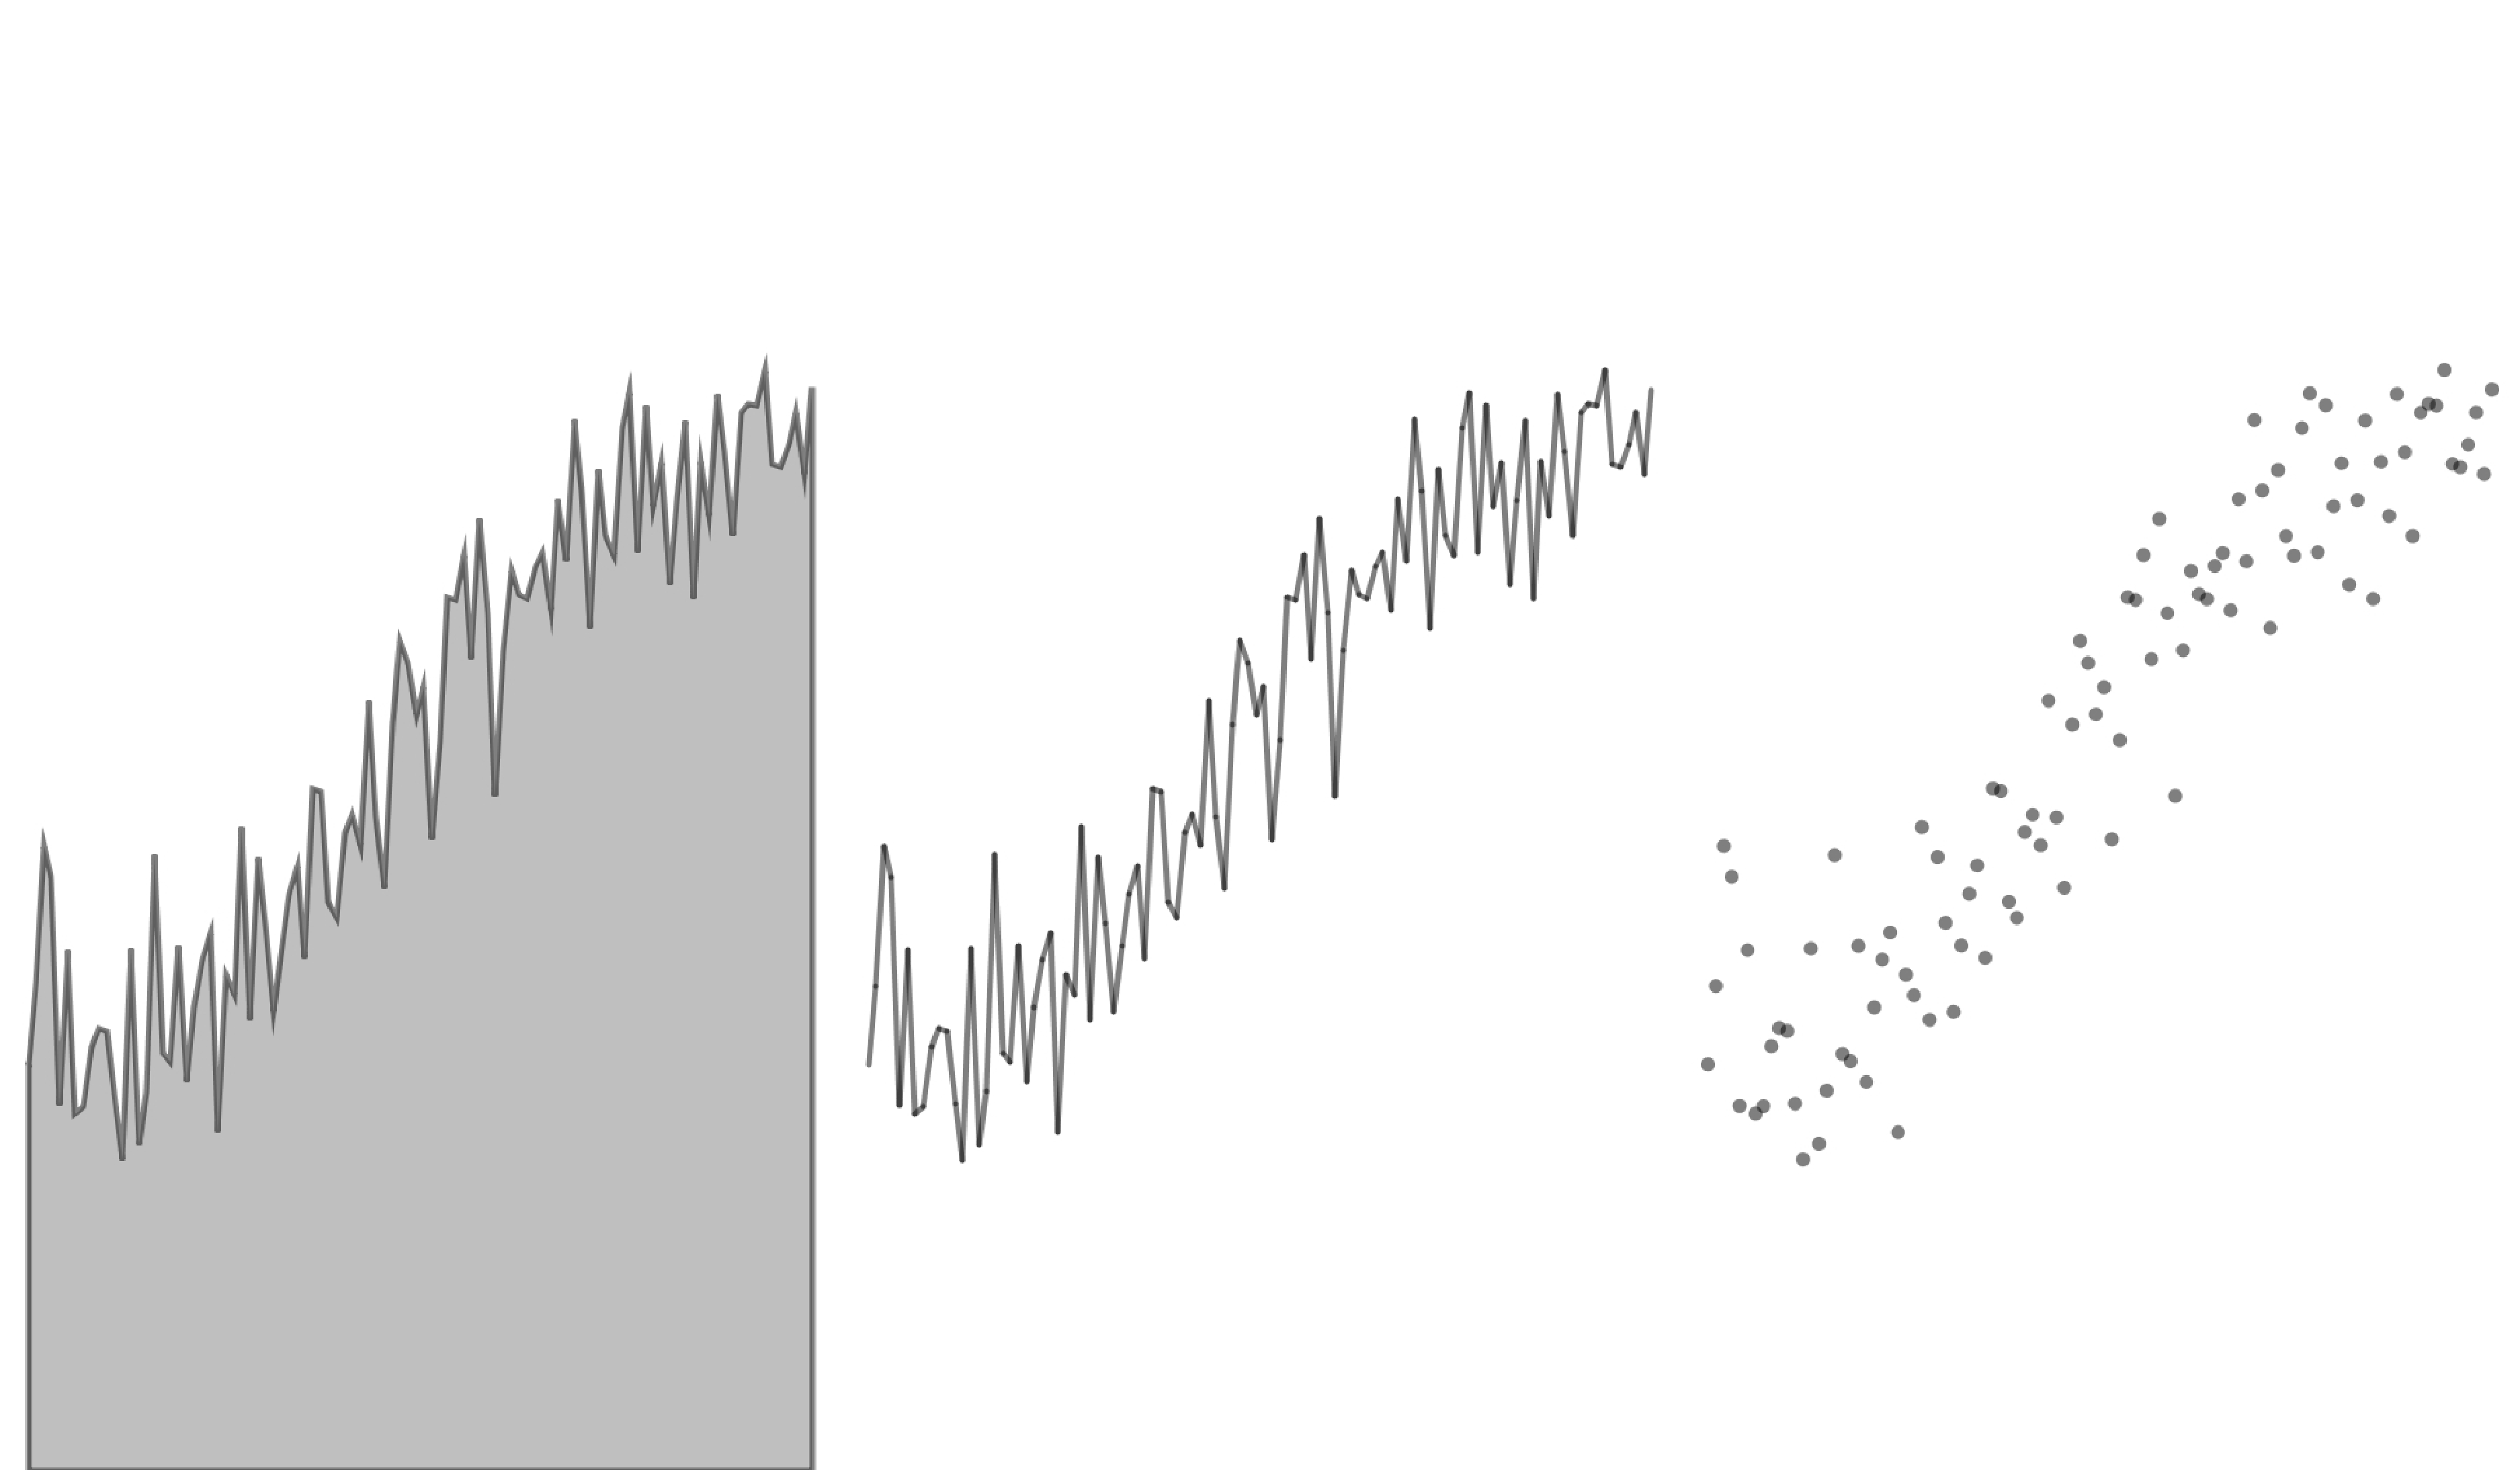
\includegraphics[width=.95\columnwidth]{figures/types}
		\caption{The three types of bivariate visualizations explored in this work: scatter plots, line graphs, and area charts. The density of points made bar charts and area charts visually similar, and so we excluded bar charts from our experiments. Likewise, the error in estimating trends from heatmaps~\protect\cite{fuchs2013evaluation} made them unsuitable for the experimental task.}
		\label{fig:types}
	\end{figure}
}

\newcommand{\expTwoTypesFig}{
	\begin{figure}
		\centering
		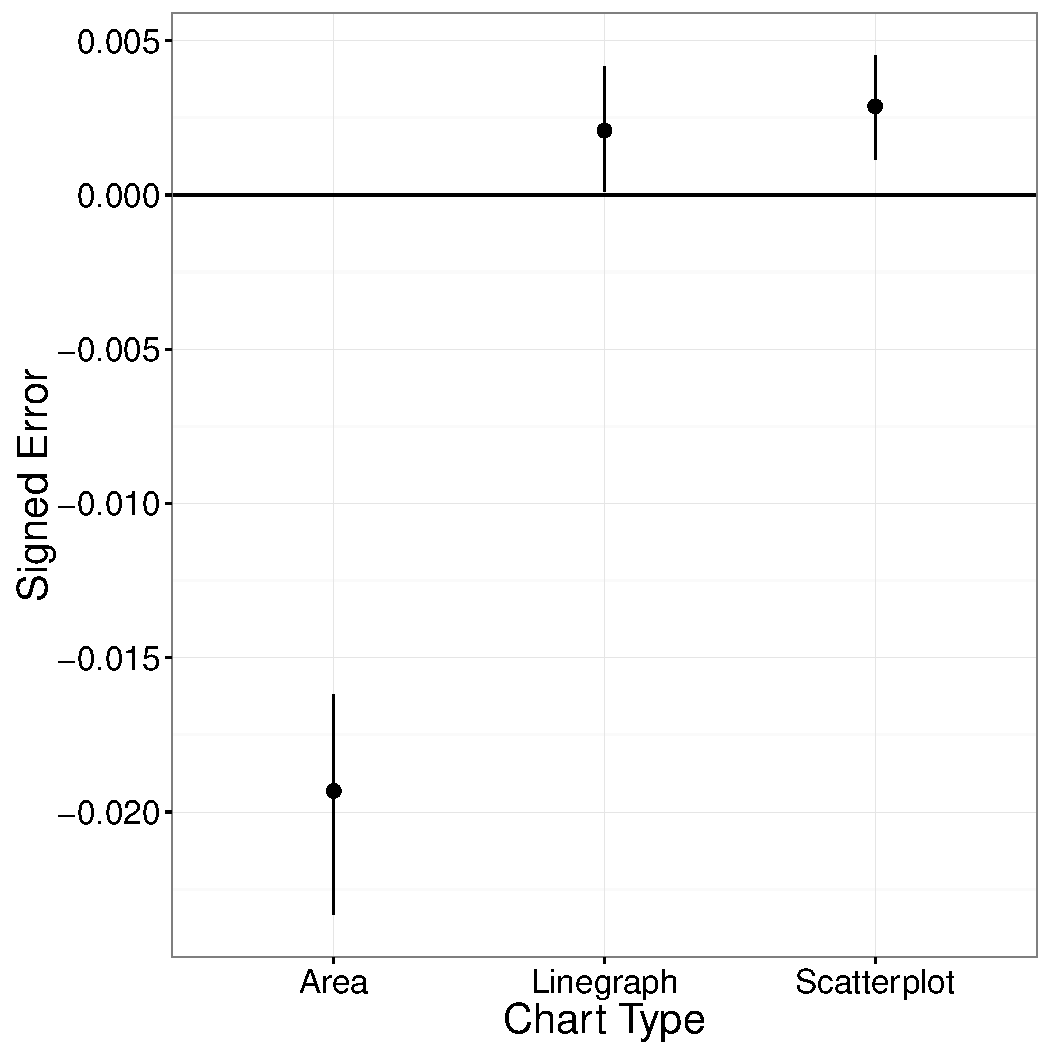
\includegraphics[width=.85\columnwidth]{figures/exp2types}
		\caption{The effect of chart type on signed error in Experiment 2. See Fig. \protect\ref{fig:sigmas} for example stimuli at each factor level. Area charts are visually asymmetric, with the area below the line filled in with a color. This visual asymmetry results in a form of within-the-bar bias~\protect\cite{newman2012bar}, where values in the filled region are perceived as likelier than values outside of it. This bias manifests as a consistent under-estimation in the intercept of trend lines. Other chart types we examined do not have this bias. Confidence intervals represent bootstrapped 95\% CIs of interquartile means. }
		\label{fig:exp2types}
	\end{figure}
}

\newcommand{\expThreeOutliersFig}{
	\begin{figure}
		\centering
		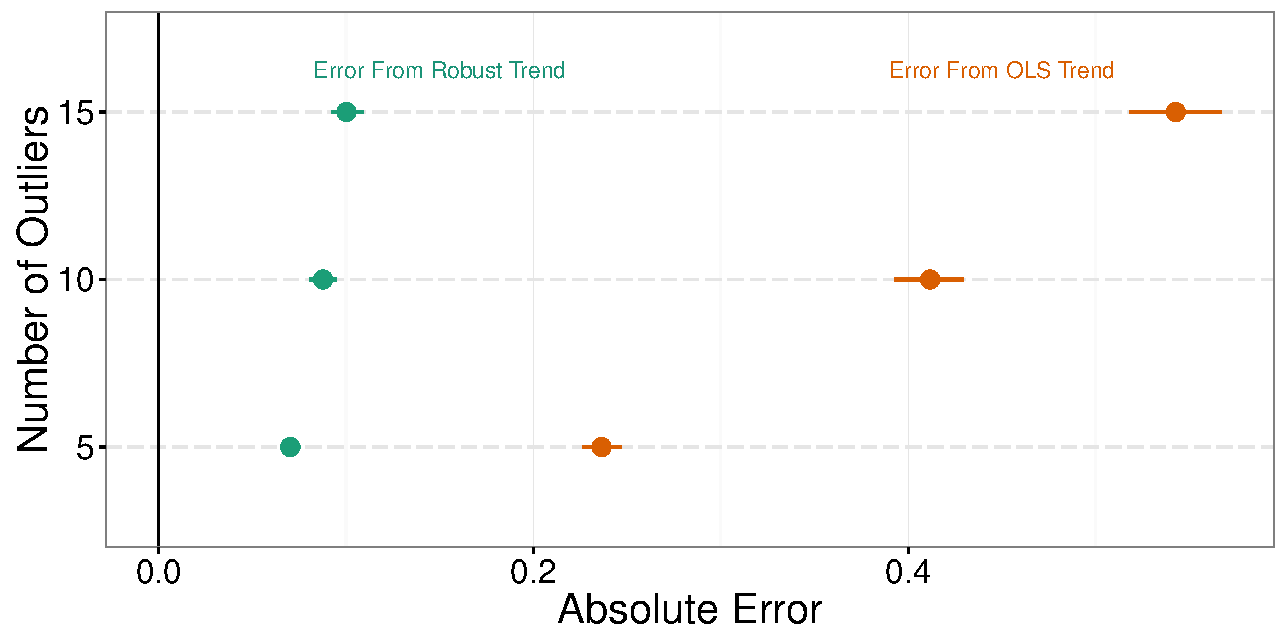
\includegraphics[width=.95\columnwidth]{figures/exp3outliers}
		\caption{The effect of numerosity of outliers on absolute error in Experiment 3. See Fig.~\protect\ref{fig:outliers} for example stimuli at each factor level. As the number of outliers increases, there is increasing divergence between the robust line of best fit (which ignores outliers), and the standard OLS line of best fit (which is sensitive to outliers). Estimates become increasingly dissimilar to the OLS fit, indicating that participants down-weight outliers when making estimates of trend. However, the increasing error even from the robust trend line indicates that participants still perform some interpolation between the two types of fits. Confidence intervals represent bootstrapped 95\% CIs of interquartile means. }
		\label{fig:exp3outliers}
	\end{figure}
}

\newcommand{\expThreeErrorFig}{
	\begin{figure}
		\centering
		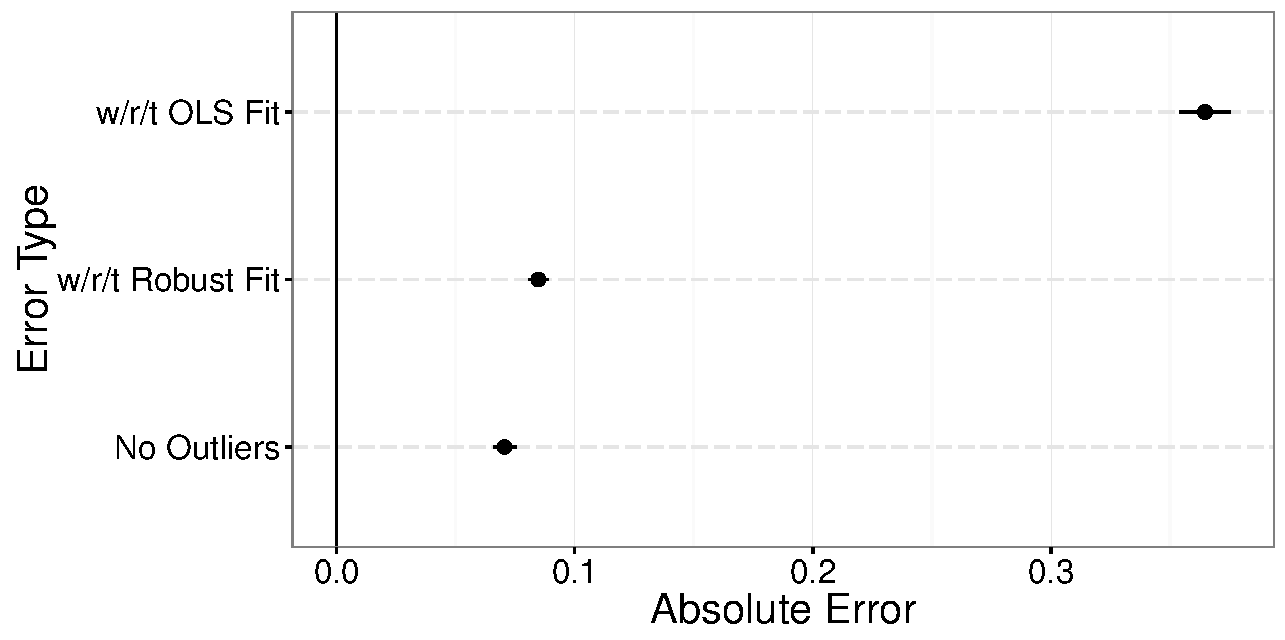
\includegraphics[width=.85\columnwidth]{figures/exp3errorType}
		\caption{The absolute error of trend estimates in Experiment 3, measured as difference from the OLS slope (which includes outliers, row 1) or from the robust slope (which excludes outliers, row 2). Participants were significantly closer to the robust fit, indicating that they were largely insensitive to outliers. We also include the absolute error for trials with no outliers for reference. Error to the robust line is higher than this standard, indicating that participants were at least performing some interpolation between OLS and robust fits, even if they largely favored the robust fit. Confidence intervals represent bootstrapped 95\% CIs of interquartile means.}
		\label{fig:exp3errorType}
	\end{figure}
}